\section{Durchführung}
\label{sec:Durchführung}
In diesem Versuch werden, wie in \autoref{sec:Ziel} bereits beschrieben, für verschiedene Spulenkonstellationen die Magnetfelder gemessen. Um diesen Versuch durchzuführen werden
allerdings vorbereitend noch ein paar wichtige Informationen gegeben.
\subsection{Vorbereitungsaufgaben}
\label{subsec:VBA}
Zunächst wird nochmals die Berechnungsformel für das Magnetfeld im Zentrum eines Helmholtzspulenpaares besprochen. Diese kann !!!!!!!!!autoref{eqn:HIERKOMMTHELOMHOLTZFORMEL REIN AUS THEORIE DU ARSCH}
entnommen werden. Sie wird durch die Geometrie eines Helmholtzspulenpaares mit dem Biot-Savart-Gesetzt(!!!!!!!eqnref{bitsavartkackereferenzmachen}) hergeleitet. Nun wird die !!!!!!!!!!!autoref{HELMSCHMOLTZREFERENZ}
anhand eines Beispiels angewendet. Dafür wird ein Helmholtzspulenpaar dessen Durchmesser $d = 125\unit{\milli\metre}$ beträgt und es gilt $\frac{d}{2} = R = x$. Das Spulenpaar 
wird von $1\unit{\ampere}$ durchflossen und die magnetische Feldkonstante $\mu_0 = 1.2566\cdot 10^{-6} \unit{\newton\per\ampere\squared}$. Setzt man diese Werte in die Gleichung ein
ergibt sich $B(0) = 0.71\unit{\milli\tesla}$ für das Magnetfeld. 


Weiter werden noch kompakt unterschiedliche Arten des Magnetismus erklärt. 
\subsubsection{Diamagnetismus}
\label{subsubsec:DIA}
Diamagnetische Stoffe sind durch eine Permeabilität $\mu_{\text{r}} < 1$ ausgezeichnet. Sie bilden unter äußerem anliegenden Magnetfeld ein inneres Gegenfeld aus. Ohne äußeres Magnetfeld sind 
diamagnetische Stoffe nicht magnetisch. 
\subsubsection{Paramagnetismus}
\label{subsubsec:PARA}
Paramagnetische Stoffe sind gewisser weise die Gegenstücke zu diamagnetischen. Sie sind ohne äußeres Magnetfeld zwar ebenfalls nicht magnetisch, aber unter Einfluss eines äußeren 
Magnetfeldes bauen paramagnetische Stoffe eine paralleles Feld zum Äußeren auf. Durch das gültige Superpositionsprinzip, welches aussagt dass in diesem Falle verschiedene Magnetfelder
überlagert werden können, ist das Feld im Inneren des Stoffes stärker. Dadurch werden sie meist in Magnetfelder hineingezogen. Paramagnetische Stoffen zeichnen sich durch eine 
Permeabilität $\mu_{\text{r}} > 1$ aus. 
\subsubsection{Ferromagnetismus}
\label{subsubsec:FERRO}
Ferromagnetische Stoffe können, ohne ein äußeres Magnetfeld, eigene permanente Mangetfelder besitzen. Diese bilden sich, da die einzelnen Atome jeweils magnetische Momente besitzen, welche 
dazu neigen sich parallel zueinander auszurichten. Die ferromagnetischen Stoffe, die kein Magnetfeld besitzen, werden meist sehr stark von einem äußeren Pol angezogen. Solche Stoffe 
sind durch eine Permeabilität $\mu_{\text{r}} >> 1$ gekennzeichnet. Eine weitere wichtige Eigenschaft solcher Stoffe ist, dass sie sich magnetisieren lassen. Diese Magnetisierung findet
durch ein äußeres Magnetfeld statt und bewirkt, dass ein ferromagnetischer Stoff sein eigenes Magnetfeld aufbaut oder verändert. Hysteresekurven, wie zum Beispiel die in \autoref{fig:PlotHysterese},
geben die Magnetisierung gegen eine gewissen Größe an. In diesem Fall wird sie gegen den Strom angegeben.
\subsection{Messung des Magnetfeldes einer langen Spule}
\label{subsec:D_Lange_Spule}
\begin{figure}
    \centering
    \caption{Bild der verwendeten langen Spule}
    \label{fig:Aufbau_lange_Spule}
    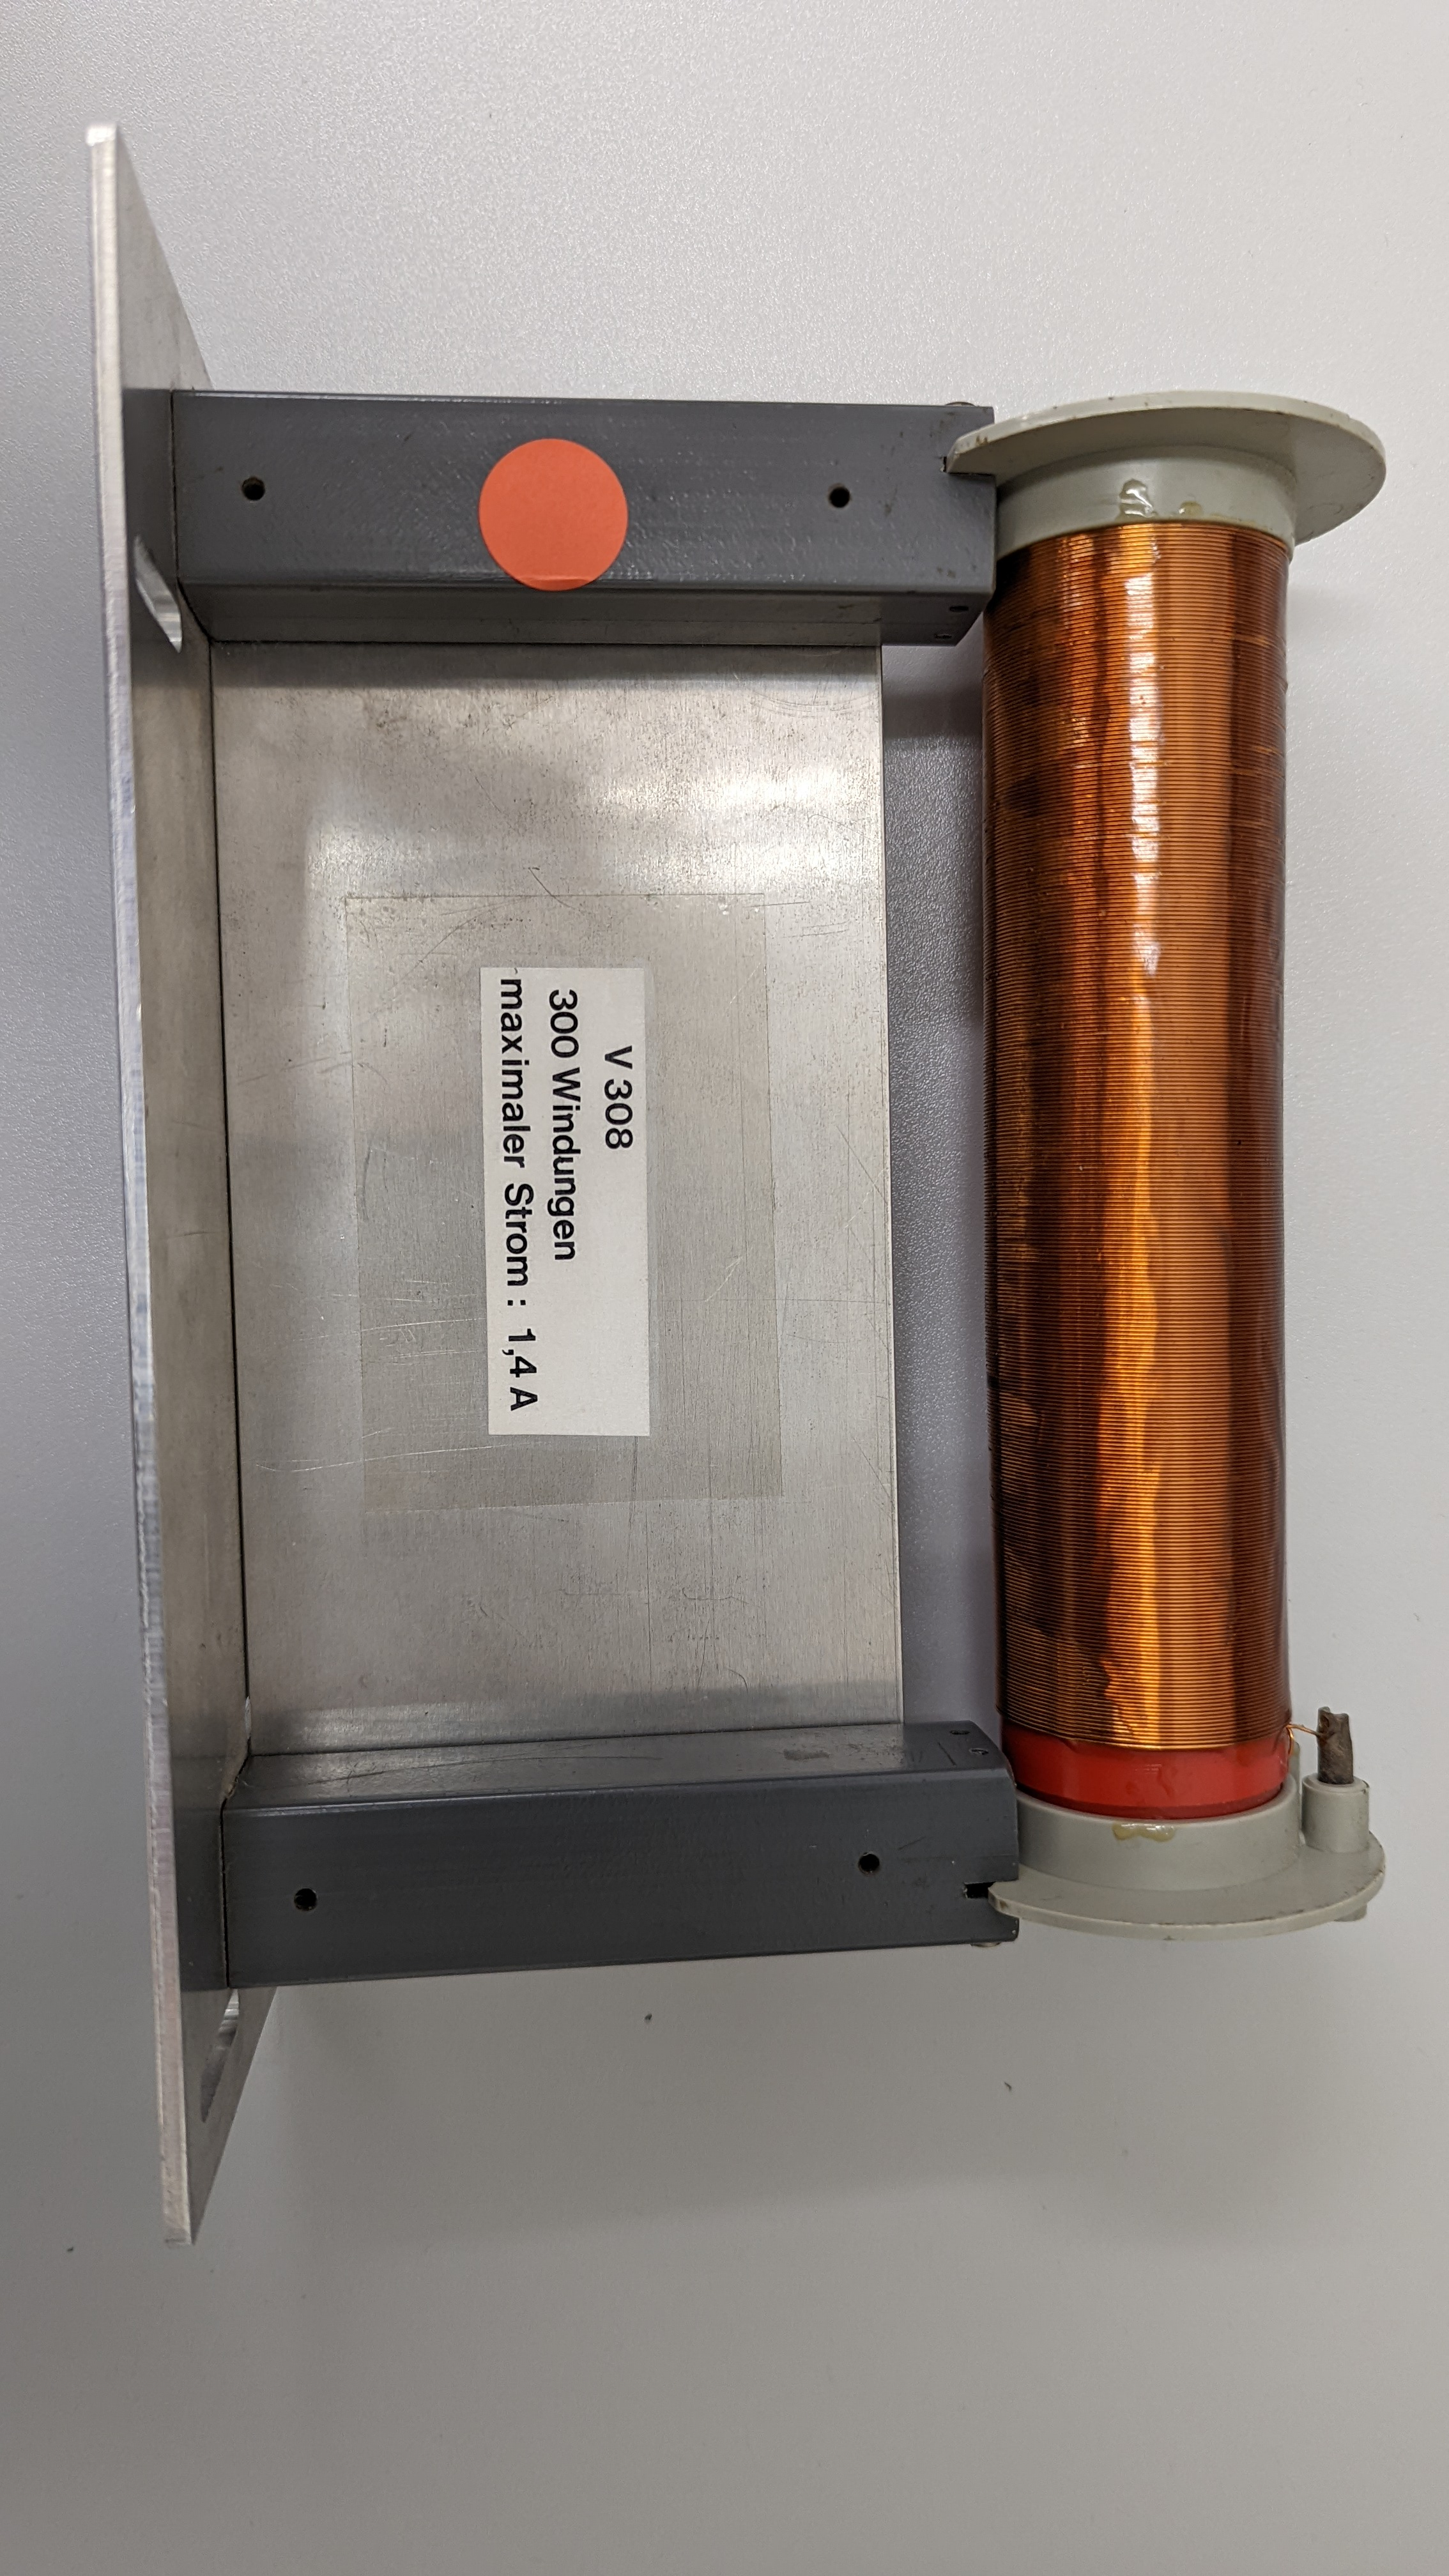
\includegraphics[width=0.55\textwidth,angle=90]{content/LangeSpule.jpg}
\end{figure}
Zur Messung des Magnetfeldes einer langen Spule benötigt man die Spule selbst, eine logitudinale Hall-Sonde und ein Stromgenerator. Zunächst wird die Spule an den Generator angeschlossen.
Der Generator wird dann so eingestellt, dass die Spule von circa $1 \unit{\ampere}$ durchflossen wird. Dann befestigt man die Hall-Sonde in einem Gestell, sodass immer möglichst auf der
gleichen Achse gemessen wird. Man wählt einem Messnullpunkt und schiebt die Hallsonde dann langsam in die Spule ein. Dabei wird die relative Auslenkung zum Messnullpunkt und die Magnetfeldstärke 
an diesen Stellen gemessen. Aus Symetriegründen reicht es aus bis zur Mitte der Spule zu messen. 
\subsection{Messung des Magnetfelds eines Spulenpaares}
\label{D_Spulenpaar}
\begin{figure}
    \centering
    \caption{Bild des verwendeten Spulenpaares}
    \label{fig:Aufbau_Spulenpaar}
    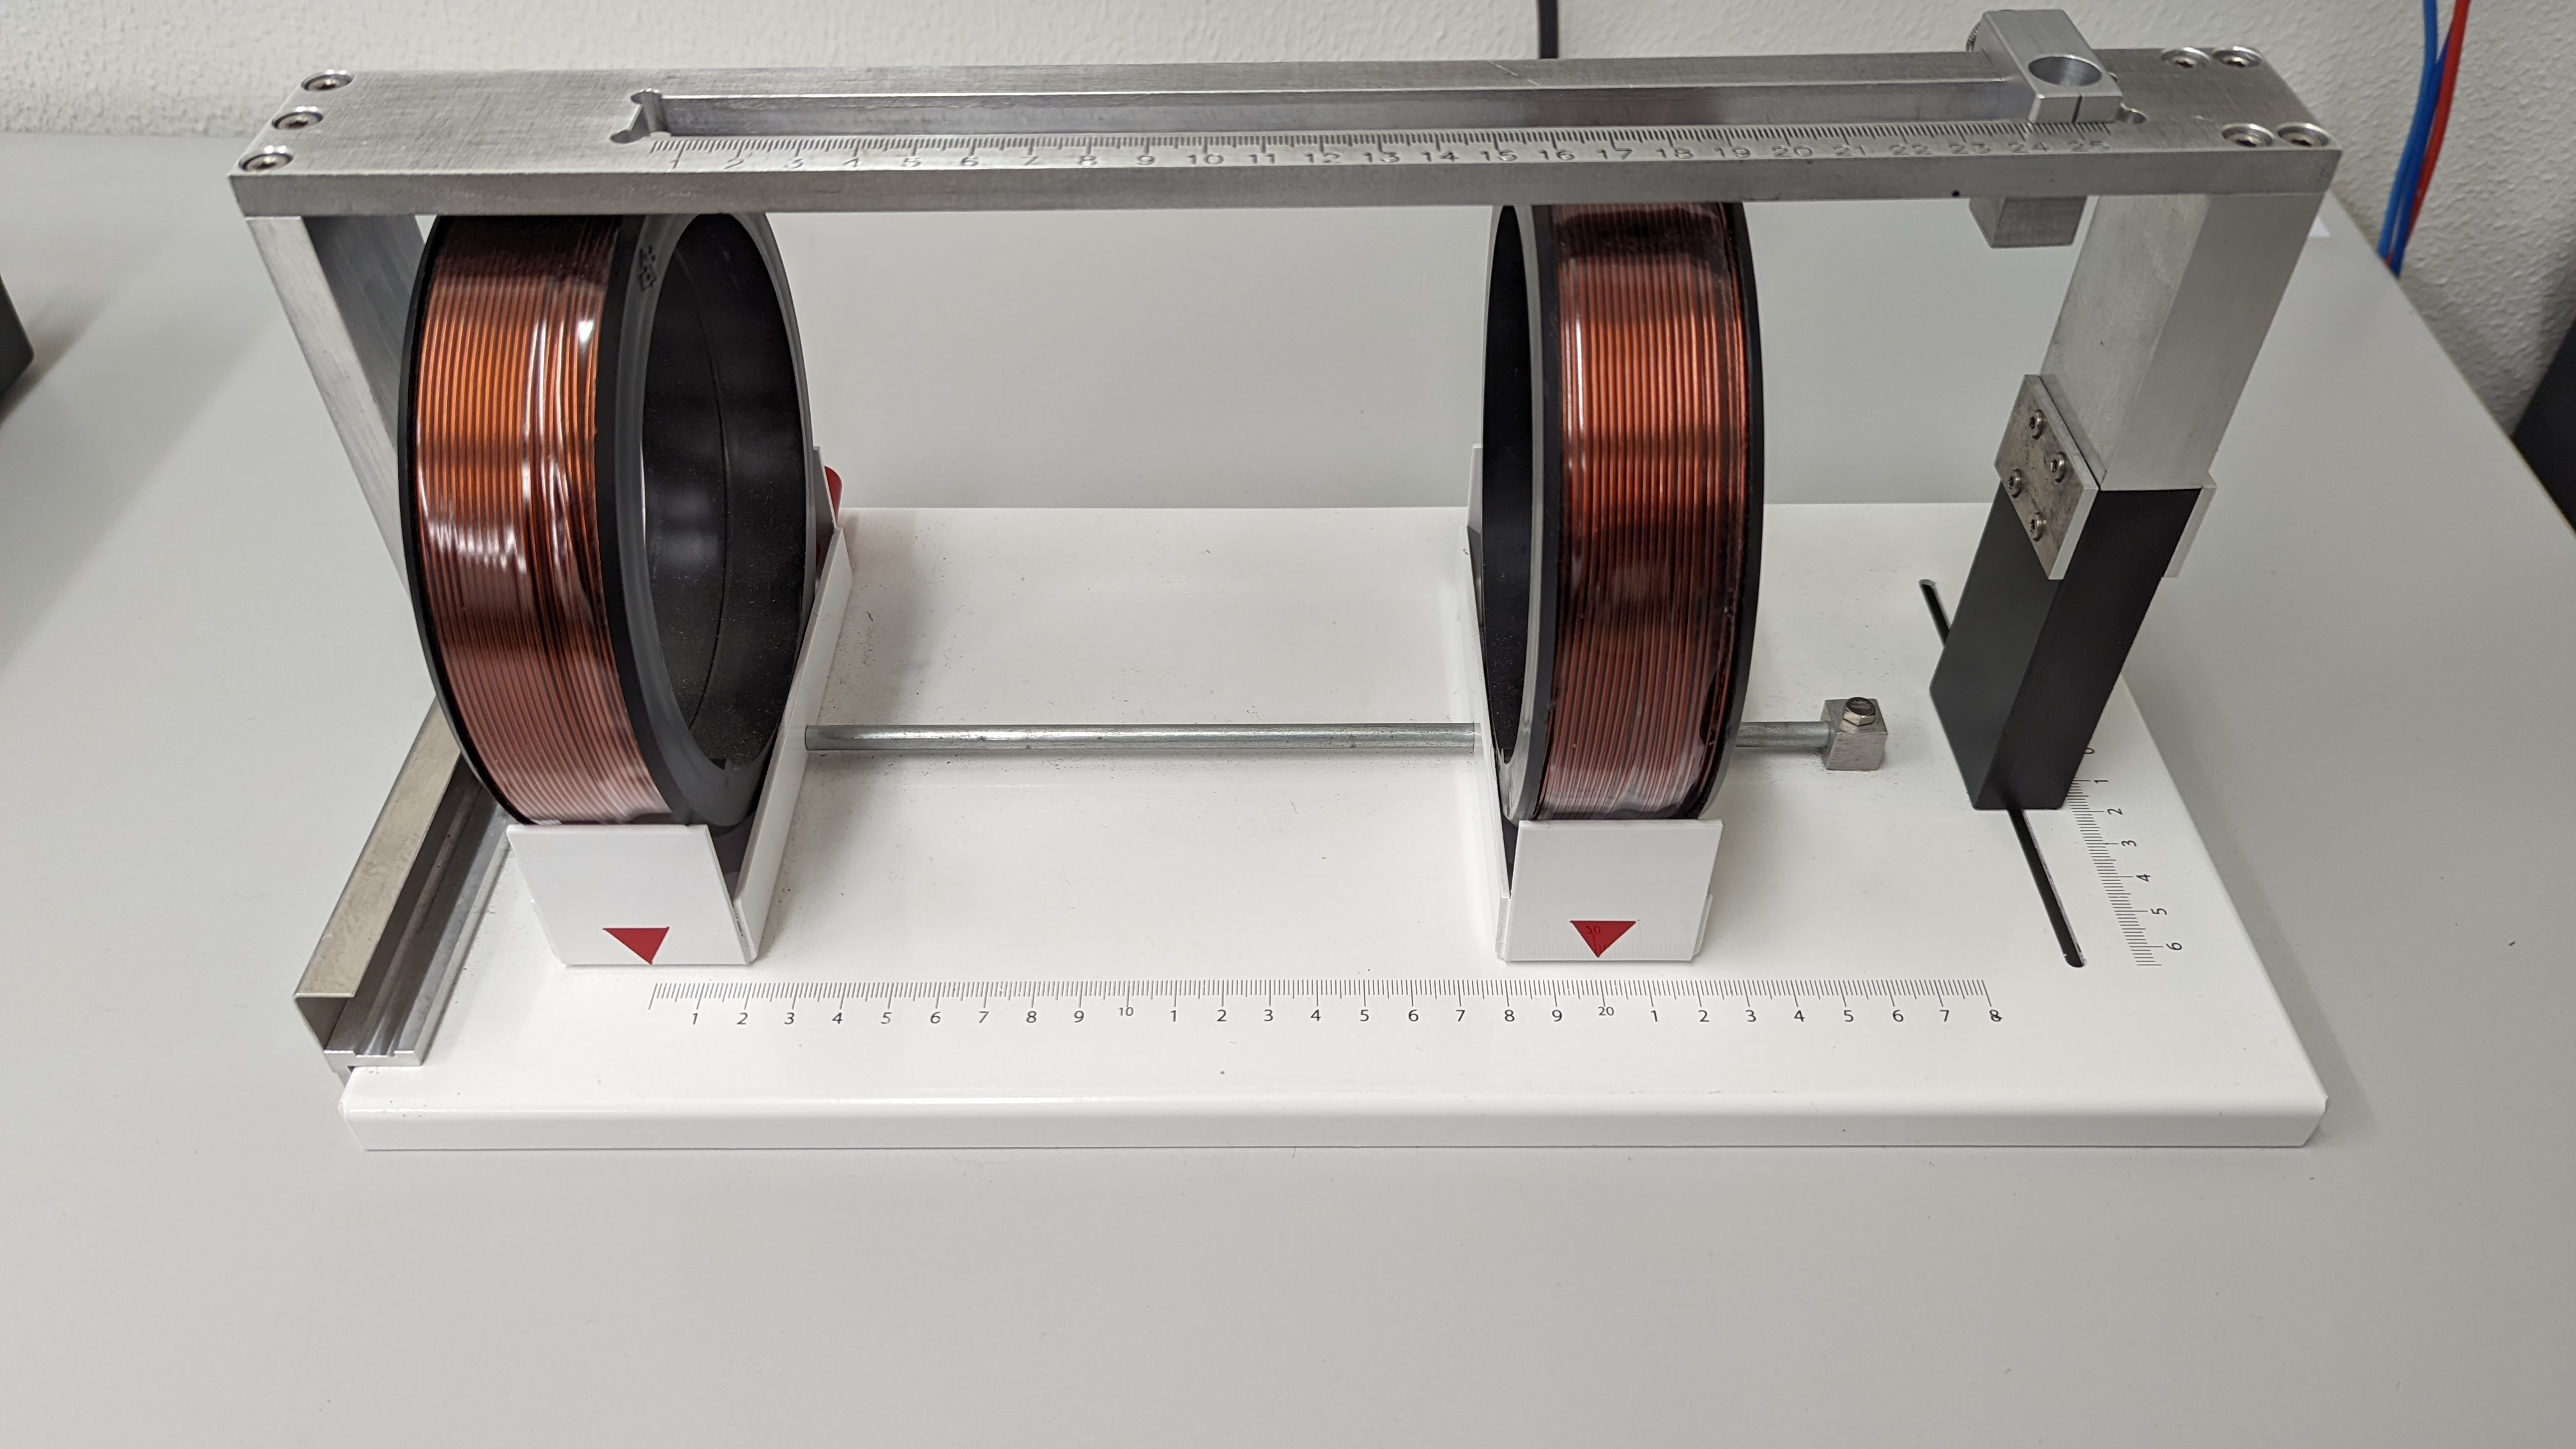
\includegraphics[width=\textwidth]{content/HelmholtzSpule.jpg}
\end{figure}
